\documentclass{article}
\usepackage[utf8]{inputenc} % Added to handle UTF-8 encoding
\usepackage{amsmath, amssymb, tikz, geometry, multicol}
\usetikzlibrary{calc}
\geometry{margin=0.25in}

\begin{document}

\begin{multicols}{2}

\section*{Trigonometry}
\begin{center}
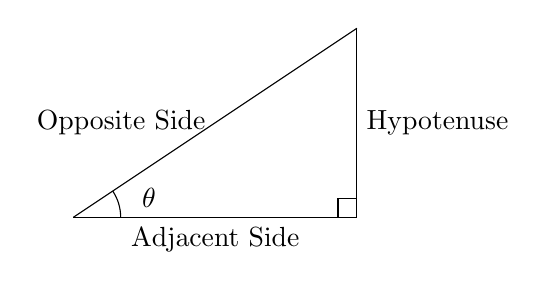
\begin{tikzpicture}[scale=1.2]
    \coordinate (A) at (0,0);
    \coordinate (B) at (3,0);
    \coordinate (C) at (3,2);
    \draw (A) -- node[below] {Adjacent Side} (B);
    \draw (A) -- node[left] {Opposite Side} (C);
    \draw (B) -- node[right] {Hypotenuse} (C);
    \draw (A) ++(0.5,0) arc (0:33.69:0.5cm);
    \node at (0.8,0.2) {\(\theta\)};
    % Right angle symbol
    \draw (B) ++(-0.2,0) -- ++(0,0.2) -- ++(0.2,0);
\end{tikzpicture}
\end{center}
\[
\sin \theta = \dfrac{\text{Opposite}}{\text{Hypotenuse}}, \quad \cos \theta = \dfrac{\text{Adjacent}}{\text{Hypotenuse}}, \quad \tan \theta = \dfrac{\text{Opposite}}{\text{Adjacent}}
\]
\[
\tan \theta = \dfrac{\sin \theta}{\cos \theta}, \quad \csc \theta = \dfrac{1}{\sin \theta}, \quad \sec \theta = \dfrac{1}{\cos \theta}, \quad \cot \theta = \dfrac{1}{\tan \theta}
\]

\section*{Unit Circle Diagram}
\begin{center}
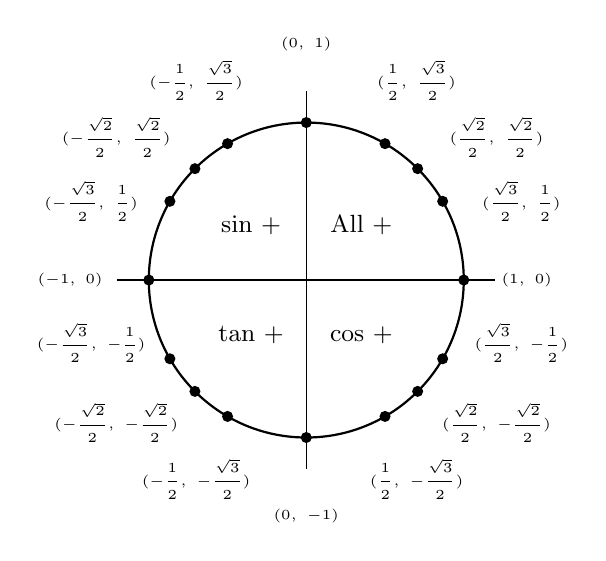
\begin{tikzpicture}[scale=2] % Increased scale for better readability
    % Draw the unit circle
    \draw[thick] (0,0) circle (1cm);
    % Axes
    \draw (-1.2,0) -- (1.2,0);
    \draw (0,-1.2) -- (0,1.2);
    % Points at common angles with labels
    \foreach \a/\d/\cs/\sn/\dx/\dy in {
        0/0^\circ/1/0/0.4/0.0,
        30/30^\circ/\dfrac{\sqrt{3}}{2}/\dfrac{1}{2}/0.5/0,
        45/45^\circ/\dfrac{\sqrt{2}}{2}/\dfrac{\sqrt{2}}{2}/0.5/0.2,
        60/60^\circ/\dfrac{1}{2}/\dfrac{\sqrt{3}}{2}/0.2/0.4,
        90/90^\circ/0/1/0.0/0.5,
        120/120^\circ/-\dfrac{1}{2}/\dfrac{\sqrt{3}}{2}/-0.2/0.4,
        135/135^\circ/-\dfrac{\sqrt{2}}{2}/\dfrac{\sqrt{2}}{2}/-0.5/0.2,
        150/150^\circ/-\dfrac{\sqrt{3}}{2}/\dfrac{1}{2}/-0.5/0,
        180/180^\circ/-1/0/-0.5/0.0,
        210/210^\circ/-\dfrac{\sqrt{3}}{2}/-\dfrac{1}{2}/-0.5/0.1,
        225/225^\circ/-\dfrac{\sqrt{2}}{2}/-\dfrac{\sqrt{2}}{2}/-0.5/-0.2,
        240/240^\circ/-\dfrac{1}{2}/-\dfrac{\sqrt{3}}{2}/-0.2/-0.4,
        270/270^\circ/0/-1/0.0/-0.5,
        300/300^\circ/\dfrac{1}{2}/-\dfrac{\sqrt{3}}{2}/0.2/-0.4,
        315/315^\circ/\dfrac{\sqrt{2}}{2}/-\dfrac{\sqrt{2}}{2}/0.5/-0.2,
        330/330^\circ/\dfrac{\sqrt{3}}{2}/-\dfrac{1}{2}/0.5/0.1
    } {
        % Calculate coordinates
        \coordinate (P) at ({cos(\a)},{sin(\a)});
        % Draw point
        \fill (P) circle (1pt);
        % Label coordinates
        \node[font=\tiny, anchor=center] at ($(P)+(\dx,\dy)$) {$(\cs,\ \sn)$};
    }
    % Quadrants
    \node at (0.35,0.35) {\small All $+$};
    \node at (-0.35,0.35) {\small $\sin$ $+$};
    \node at (-0.35,-0.35) {\small $\tan$ $+$};
    \node at (0.35,-0.35) {\small $\cos$ $+$};
\end{tikzpicture}

The cosine is the x-value, the sine is the y-value

\textbf{Radians to Degrees Conversion}
\[
180^\circ = \pi \text{ radians}, \quad 1^\circ = \dfrac{\pi}{180} \text{ radians}
\]

For common angles, sine and cosine values can be calculated as:
\[
\sin \theta = \dfrac{\sqrt{n}}{2}, \quad \cos \theta = \dfrac{\sqrt{4 - n}}{2}
\]
where \( n \) corresponds to the following angles:
\begin{center}
\begin{tabular}{ll}
\( n = 0 \) & for \( \theta = 0^\circ \), \\
\( n = 1 \) & for \( \theta = 30^\circ \), \\
\( n = 2 \) & for \( \theta = 45^\circ \), \\
\( n = 3 \) & for \( \theta = 60^\circ \), \\
\( n = 4 \) & for \( \theta = 90^\circ \). \\
\end{tabular}
\end{center}

\end{center}

\section*{Pythagorean Identity}
\[
\sin^2 \theta + \cos^2 \theta = 1
\]
\textbf{Example Calculation:} If \( \sin \theta = \dfrac{3}{5} \), then:
\[
\cos \theta = \sqrt{1 - \left( \dfrac{3}{5} \right)^2} = \dfrac{4}{5}
\]

\columnbreak

\section*{Addition Formulas}

\subsection*{Sine Addition and Subtraction Formulas}
\[
\sin(A \pm B) = \sin A \cos B \pm \cos A \sin B
\]

\subsection*{Cosine Addition and Subtraction Formulas}
\[
\cos(A \pm B) = \cos A \cos B \mp \sin A \sin B
\]

\section*{Law of Sines}
\begin{center}
\begin{tikzpicture}[scale=1.2]
    \coordinate (A) at (0,0);
    \coordinate (B) at (3,0);
    \coordinate (C) at (1.5,2.5);
    \draw (A) -- node[below] {$c$} (B) -- node[right] {$a$} (C) -- node[left] {$b$} (A);
    \node[below left] at (A) {$A$};
    \node[below right] at (B) {$B$};
    \node[above] at (C) {$C$};
\end{tikzpicture}
\end{center}
\[
\frac{\sin A}{a} = \frac{\sin B}{b} = \frac{\sin C}{c}
\]
\textbf{Inverse Formulation:}
\[
\frac{a}{\sin A} = \frac{b}{\sin B} = \frac{c}{\sin C}
\]
\textbf{Example Calculation:} If \( a = 7 \), \( A = 30^\circ \), and \( B = 45^\circ \), find \( b \):
\begin{align*}
\frac{a}{\sin A} &= \frac{b}{\sin B} \\
b &= a \times \frac{\sin B}{\sin A} \\
&= 7 \times \frac{\sin 45^\circ}{\sin 30^\circ} \\
&= 7 \times \frac{\frac{\sqrt{2}}{2}}{\frac{1}{2}} \\
&= 7 \times \sqrt{2} \approx 9.9
\end{align*}

\section*{Law of Cosines}
\[
a^2 = b^2 + c^2 - 2bc \cos A
\]
\textbf{Example Calculation:} Given \( b = 5 \), \( c = 7 \), and \( A = 60^\circ \):
\begin{align*}
a^2 &= 5^2 + 7^2 - 2 \times 5 \times 7 \times \cos 60^\circ \\
&= 25 + 49 - 70 \times \left( \dfrac{1}{2} \right) \\
&= 74 - 35 \\
&= 39 \\
a &= \sqrt{39} \approx 6.24
\end{align*}

\section*{Area of a General Triangle}
\[
\text{Area} = \dfrac{1}{2} ab \sin C
\]

\section*{Triangle Inequality}
For any triangle with sides \( a \), \( b \), and \( c \):
\[
\begin{aligned}
a &< b + c \\
b &< a + c \\
c &< a + b
\end{aligned}
\]
\textbf{Example:} If \( a = 3 \), \( b = 4 \), then \( c \) must satisfy:
\begin{align*}
c &< 3 + 4 \implies c < 7 \\
c &> |3 - 4| \implies c > 1
\end{align*}

\end{multicols}

\end{document}
